\section{Einleitung in DevSecOps}
In der heutigen Zeit gewinnt das DevOps-Prinzip im Softwareentwicklungszyklus zunehmend an Bedeutung. DevOps fördert die Integration von Entwicklung und Betrieb und verringert die bisherige Trennung zwischen diesen Bereichen ~\cite{Sharma2013}.  Dieser Ansatz wird durch das Prinzip "'you build it, you run it"' verkörpert, welches die Verantwortlichkeit für den gesamten Lebenszyklus einer Anwendung in die Hände der Entwickler legt.

\begin{figure}[h!]
  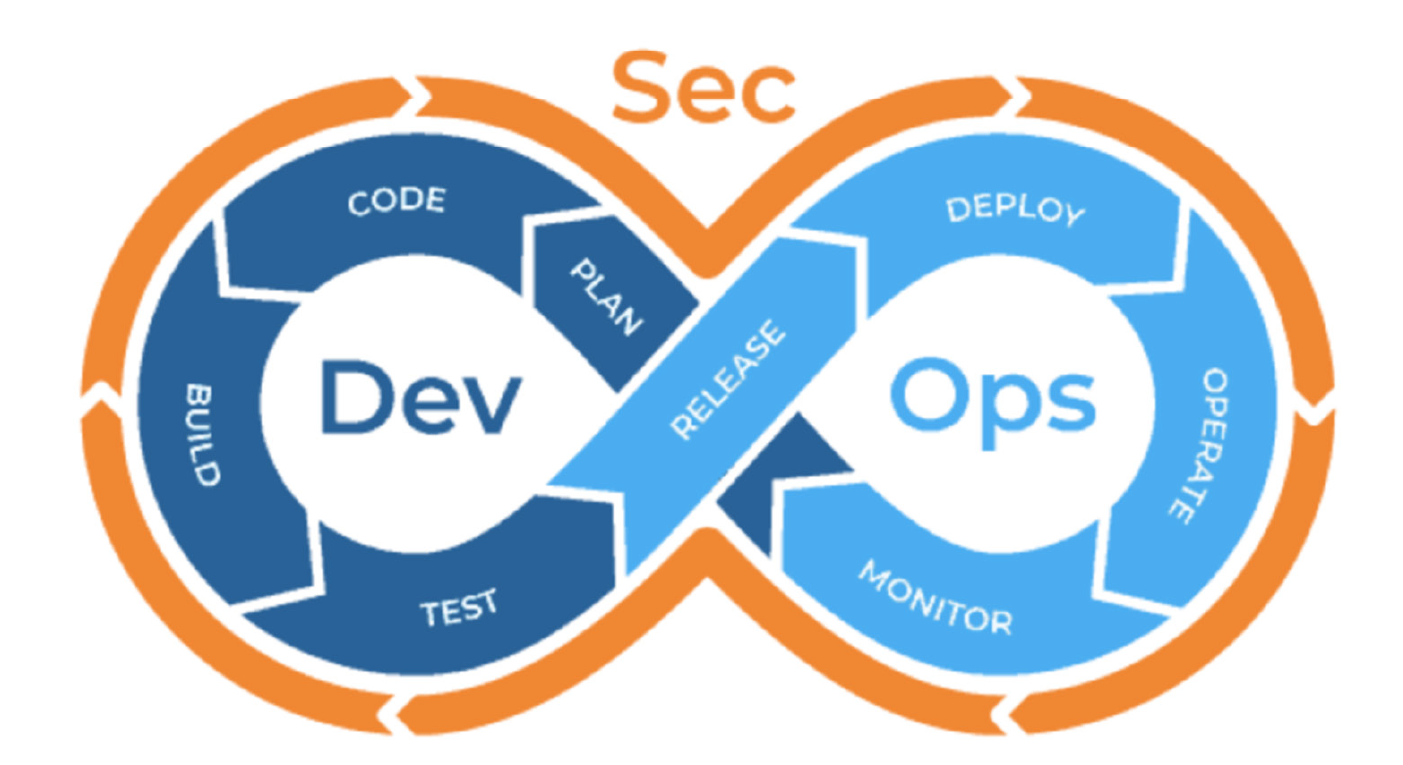
\includegraphics[width=\linewidth]{img/DevSecOps.png}
  \caption{DevSecOps Zyklus ~\cite{Haug2020}}
  \label{fig:devsecops}
\end{figure}

In traditionellen Softwareunternehmen, ist Sicherheit meist ein separater Schritt, welcher Mehraufwand und somit Kosten verursacht. In modernen DevOps orientierten Unternehmen ist dies nicht der Fall, dort wird Sicherheit als Geschäftsfaktor gesehen und somit eher als Feature mit Mehrwert anstelle einer Last~\cite{Wong2024}.

Dies ist sowohl im Hinblick auf die Vermeidung von ungeplanter Arbeit und Nacharbeit als auch während des eigentlichen Verkaufsprozesses, wenn Sicherheitsanforderungen als Teil einer Sicherheitsbewertung des Anbieters festgelegt werden, von Bedeutung.

Dieser Ansatz, Sicherheitsaspekte frühzeitig und kontinuierlich in den Softwareentwicklungsprozess zu integrieren, wird als "'shift left"' bezeichnet. Dies bedeutet, dass Sicherheitsmaßnahmen nicht erst am Ende des Produktzyklus, sondern bereits während der Entwicklung berücksichtigt werden müssen ~\cite{Haug2020}.

\begin{figure}[h!]
  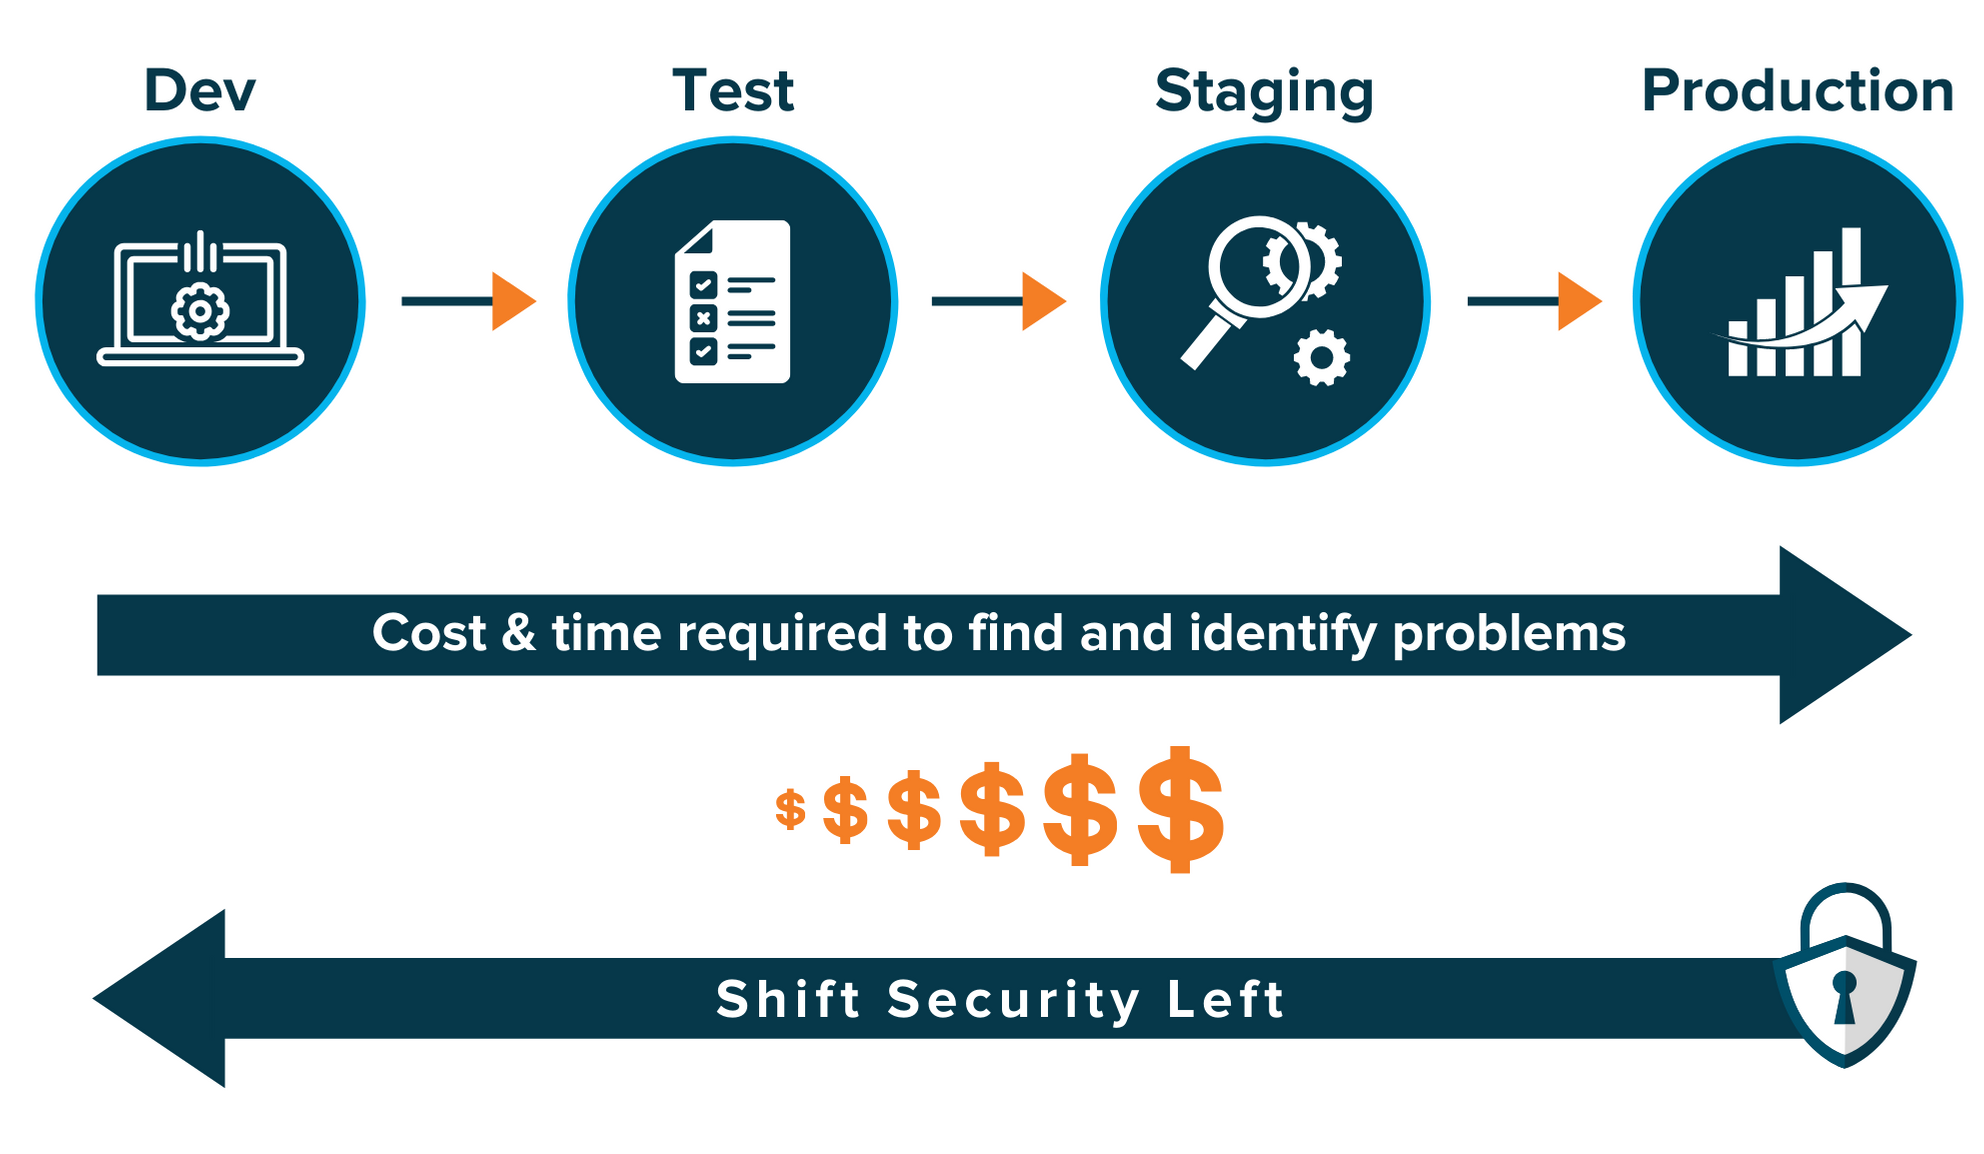
\includegraphics[width=\linewidth]{img/ShiftLeft.png}
  \caption{Shift Left der Sicherheit ~\cite{Haug2020}}
  \label{fig:shiftleft}
\end{figure}

In dieser Arbeit liegt der Schwerpunkt auf der Implementierung von Quality Gates, die darauf abzielen, die Sicherheit von Software zu erhöhen. Insbesondere wird der Fokus auf das Dependency Scanning zur Identifikation bekannter Sicherheitslücken und die statische Code-Analyse gelegt, um potenzielle Fehler und Schwachstellen im Code frühzeitig zu erkennen.

Durch diese Maßnahmen wird nicht nur die Sicherheit der Software verbessert, sondern auch die Effizienz des gesamten Entwicklungsprozesses gesteigert. Die Bedeutung dieser Ansätze wird im Kontext moderner Softwareentwicklung erläutert und durch praxisnahe Beispiele und Fallstudien untermauert.


Diese Arbeit richtet sich an Software-Entwickler und IT-Fachleute, die DevOps und DevSecOps einführen möchten. Ziel ist es, die Sicherheit und Qualität ihrer Software-Releases zu verbessern. Leser sollten grundlegendes Wissen über Softwareentwicklung und IT-Betrieb haben und daran interessiert sein, Sicherheits- und Qualitätsstrategien sowie Security-Gates in ihren Entwicklungsprozess zu integrieren. Die Arbeit bietet anhand von zwei Beispielen eine Implementierung sowie Best Practices, um eine sichere und effiziente  Softwareentwicklung zu gewährleisten.